
\chapter{Graph Matching}

In this chapter we review basic definitions and notations from the graph theory used in this thesis and introduce different forms and formulations of the graph matching problem together with some algorithms for solving them. The classification we use is based on~\cite{Conte2004}, although we concentrated our attention mainly on one specific group of algorithms: those, which consider the graph matching problem as a quadratic optimization problem. Not all algorithms, we present thereby, were initially mentioned in~\cite{Conte2004}, but we also do not cover all of the resent ones due to their quantity. We focus our selfs specially on those, that are important for further reading of the thesis.

\section{Basic definitions and notation}
A \emph{undirected graph} $G=(V,E)$ is defined as a pair of disjoint sets $V$, $E$, where $E\subseteq\{\{u,v\}| u, v\in V\}$~\cite{Diestel2000}. The elements of the set $V$ are called \emph{vertices} or \emph{nodes}\footnote{We use terms vertex and node further in the text as synonyms} and the elements of $E$ are called \emph{edges}. Where it is necessary, we will write $V(G), E(G)$ to refer node and edge sets to the graph $G$.

The number of nodes in $V$ defines the \emph{size} of a graph $G$.
Two nodes $v_{i},v_{i'}\in V$ are called \emph{adjacent}, if there is an edge $e=\{v_{i},v_{i'}\}\in E$. Each graph can be represented by its \emph{adjacency matrix A=$(a_{ij})_{n\times n}$}, where 
\begin{equation*}\centering
a_{ij}=\begin{cases}
 1, & \text{if } \{v_{i},v_{i'}\}\in E, \\
 0, & \text{otherwise.} \\
\end{cases}
\end{equation*}
and $n$ is the number of nodes in the graph.

A \emph{path} in a graph $G=(V,E)$ is a sequence of nodes $\{v_0,v_1,\dots,v_k\}$ connected by the edges $\{v_0v_1,v_1v_2,\dots,v_{k-1}v_k\}$, where $v_i\in V$ and $v_{i-1}v_i\in E$ for all $i=0,\dots,k$. A path with $v_0=v_k$ is a \emph{cycle}.

A graph $G'=(V',E')$ is called a \emph{subgraph} of a graph $G=(V,E)$, if $V'\subseteq V$ and $E'\subseteq E$. We use the standard notation $G'\subseteq G$ for this. The subgraph $G'$ of $G$ is \emph{induced by the set $V'\subseteq V$}, if $E'=\{(v_i, v_{i'})|v_i,v_{i'}\in V'\}$. Analog, the set $E'\subseteq E$ induces the subgraph $G'$ of $G$, if $V'=\{v\in V|v\in e\text{ and }e\in E'\}$. For the induced subgraph we use the notation $G'=G[V']$ and $G'=G[E']$~\cite{Diestel2000}, depending if it is node- or vertex-induced. We also define graph cut $G\cap G'=(V\cap V', E\cap E')$ and union $G\cup G'=(V\cup V', E\cup E')$.

There are several special types of graphs. A graph, whose each pair of nodes is connected by an edge is called \emph{complete}. In case, when each node $v_i\in V$ of a graph $G$ has an associated attribute $d_i\in D$, one speaks about \emph{attributed graph} $G=(V,E,D)$. If in contract to this each edge of a graph has an associated weight, the graph is called \emph{weighted graph}. A connected, undirected graph without cycles is called a \emph{tree}. A $hypergraph$ is graph, whose edges connect several vertices at the same time (\emph{hyperedges}).

Consider two undirected attributed graphs $G^I = (V^I, E^I, D^I)$ and $G^J = (V^J, E^J,\newline D^J)$. We assume the situation, where $|V^I|=n_1$, $|V^J|=n_2$ and $n_1\le n_2$. A \emph{matching function} between $G^I$ and $G^J$ is a mapping $m:V^I\rightarrow V^J$ between the sets of nodes of two graphs.
It is clear, that defined in this way the mapping $m$ is not unique. Assume, that we have some metric $S(G^I, G^J, m)$ to measure the quality of matching $m$. In this case, \emph{Graph matching problem} between $G^I$ and $G^J$ can be defined as a problem of finding such a map $m:V^I\rightarrow V^J$, that maximizes the similarity score $S(G^I, G^J, m)$ between the graphs and fulfills some additional constraints:
\begin{equation} \label{gGMP}
m = \argmax_{\hat{m}}S(G^I, G^J, \hat{m})
\end{equation}
Based on the required properties of the mapping $m$ the algorithms, that solve this problem, can be divided into two large groups~\cite{Conte2004}: \emph{exact} and \emph{inexact} graph matching methods. There are also variations inside of each group based on the definition of the similarity score between two graphs. In the following sections we will give an overview of the common exact and inexact graph matching algorithms.
 
\section{Exact graph matching}
The group of exact graph matching algorithms represents a class of more strict methods, that require the mapping between nodes of two graphs to be \emph{edge preserving}. With other words: if $\{v_i,v_{i'}\}\in E^I$, then $\{m(v),m(v_{i'})\}\in E^J$ for all $v_i,v_{i'}\in V^I$. The graphs, considered in this case often do not have attributes.

There are several forms of the exact graph matching. The most known one is \emph{graph isomorphism}: two graphs are called \emph{isomorph} ($G^I\simeq G^J$), if the edge preserving mapping between their nodes is bijective. This implies, that two graphs have the equal number of nodes. If it is not the case, and the isomorphism holds between the one graph and a node-induced subgraph of the other graphs, the problem is called \emph{subgraph isomorphism}. Its further extension is a isomorphism between subgraphs of the graphs. The last problem can obviously have several solutions, but one is normally interested in finding a common subgraph with maximum number of nodes or edges (\emph{maximum common subgraphs}).  

The further simplification of the graph isomorphism is to require an injective edge-preserving mapping, instead of bijective. This problem is called \emph{graph monomorphism}. The correspondences here are still one-to-one, but the second graph may contain additional nodes and edges, comparing to the first graph.
Even weaker form of graph matching problem is \emph{graph homomorphism}. It allows many-to-one mapping between nodes of two graphs, which means that the only one restriction on the mapping $m$ is to be total.
On the Fig.~\ref{fig:Exact_GM} one can see examples of different exact graph matching problems.
\begin{figure}[h!]
    \centering
    \begin{subfigure}[b]{0.3\textwidth}
        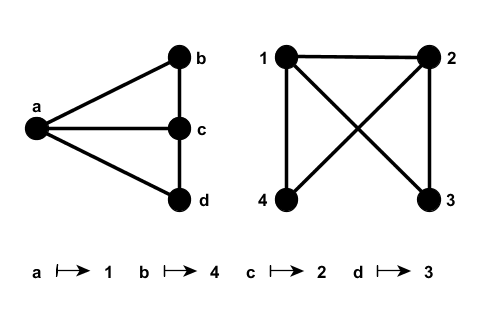
\includegraphics[width=\textwidth]{chapter1/fig/GI}
        \caption{Graph isomorphism}
        \label{fig:GI}
    \end{subfigure}
    ~
    \begin{subfigure}[b]{0.3\textwidth}
        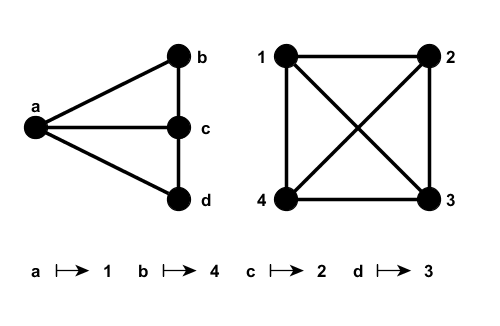
\includegraphics[width=\textwidth]{chapter1/fig/monomorphism}
        \caption{Graph monomorphism}
        \label{fig:monomorphism}
    \end{subfigure}
    ~
    \begin{subfigure}[b]{0.3\textwidth}
        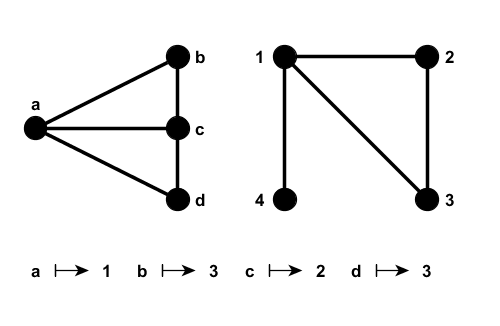
\includegraphics[width=\textwidth]{chapter1/fig/homomorphism}
        \caption{Graph homomorphism}
        \label{fig:homomorphism}
    \end{subfigure}
    \caption{Exact graph matching problems}\label{fig:Exact_GM}
\end{figure}

%\subsection{Compexity}
All problems except graph isomorphism are proofed to be $NP-$complete~\cite{Garey_NPComplet}. This can be shown through the reduction of the matching problem to the clique problem. The graph isomorphism is currently shown to be $NP-$hard~\cite{Garey_NPComplet,Schoening_GI}. For special types of graphs there exist polynomial time algorithms (e.g. for %planar graphs~\cite{Hopcroft_Wong} and 
trees~\cite{Aho_Ullman, Garey_NPComplet}).

%\subsection{Methods}
The most widespread approach to solve exact graph matching problems is based on tree search with backtracking. The idea is to starts with an empty solution and try in each step to expend it based on some rules until the solution is found. If it happens, that on some step a current solution cannot be expend further due to problem's constraints, the current branch is cut and algorithm backtracks to the last feasible solution and tries to expand it in other way. Those algorithms are very slow, if they need to search through the whole tree, but can be speeded up by applying some heuristic to detect unpromising branches and exclude them from the search. The most known algorithm in this group, which uses depth-first-rule to traverse a tree, is the branch and bound~\cite{Reingold} algorithm.

The one of the first algorithms, that uses described techniques, is the one by Ullman~\cite{Ullmann}. Later it was extended and improved mostly by the suggestion a new pruning heuristics (see for example~\cite{Lee2013} for comparison of algorithms based on the same technique). We also want to mention here another well known algorithm, which uses the tree search method and is closely related to maximal common subgraph problem, - algorithm by Bron and Kerbosch~\cite{BronKerbosch} for finding cliques in an undirected graphs.

The other techniques, that were successfully applied for the (sub)graph isomorphism are decision trees~\cite{Messmer1999,Shearer1998,Shearer2001} and group theory\cite{McKay} for maximal subgraph matching. 

\section{Inexact graph matching}

Sometimes it is difficult to apply the exact matching algorithms described in previous section to real world problems. There are two possible reasons for that. On the one hand, that are variations in the structure of graphs, that describe a same object. Those variations could be a consequence of natural deformations or noise influence, that can occur in some real word applications. On the other hand, solving the graph matching problem exactly can be time or memory consuming. As a consequence one can be interested in solving graph matching problem inexactly. In this case, no edge preserving mapping between the nodes of two graphs is required.
\begin{figure}[htb]
	\centering
	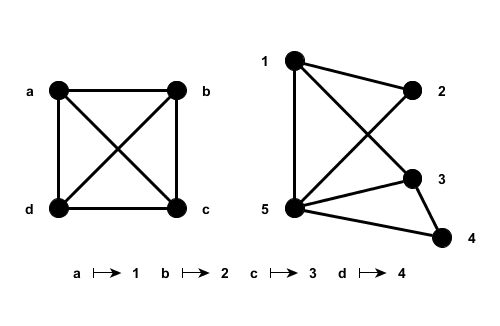
\includegraphics[width=0.5\textwidth]{chapter1/fig/inexactGM}
    \caption{Inexact graph matching}
    \label{fig:inexact_GM}
\end{figure}

Let us recall the problem statement \eqref{gGMP}: 
\begin{equation*}
m = \argmax_{\hat{m}}S(G^I, G^J, \hat{m})
\end{equation*}
where $S(G^I, G^J, \hat{m})$ defines the similarity measure between the attributed graphs $G^I = (V^I, E^I,D^I)$ and $G^J = (V^J, E^J,D^J)$. The mapping $m$ is required to be total and sometimes also injective, to guarantee one-to-one matching.

Depending if an algorithm for solving \eqref{gGMP} finds a global solution or not, it is called \emph{optimal} or \emph{suboptimal}. The choice, which algorithm to select depends on a specific problem. It should be noted, that an optimal inexact algorithms is not necessary faster than the exact one. On the other hand, suboptimal inexact algorithms often do not have any performance guarantee.

There are also different ways to define a similarity function $S(G^I,G^J,m)$, which leads to high number of different approaches inside the group of inexact graph matching algorithms. In the following section we summarized the most common form of objective function of the problem \eqref{gGMP}.

\subsection{Graph Matching Objective Function}

In some literature instead of defining the similarity function as in \eqref{gGMP} one speaks about dissimilarity between two graphs~\ToDo{cite} or matching score~\ToDo{cite}. The goal in this case is to minimize those values. Two versions of the problem formulation are however equivalent and one can easy transform one into other.

\subsubsection{Quadratic Optimization Problem}
The objective of graph matching is to find a mapping between two attributed graphs $G^I = (V^I, E^I,D^I)$ and $G^J = (V^J, E^J,D^J)$. Let the size of the graphs be $n_1$ and $n_2$ respectively. Generally, $n_1$ and $n_2$ can be different, but then we assume without losing generality $n_1\le n_2$. Here and further, we require the mapping $m$ in \eqref{gGMP} to be total and injective, which guarantees, that each node of the first graph will be matched to exactly one node of the second graph (one-to-one matching). 

We start with a even stricter assumption, that $n_1=n_2=n$ and the matching is bijective. In this case a mapping between nodes of the two graphs defines a permutation $\sigma$ of the set $\{1,\dots,n\}$. Each permutation $\sigma$ can be represented by the permutation matrix $P=\{P_{ij}\}$, where
\begin{equation*}
P_{ij}=\begin{cases}
 1, & \text{if } \sigma(i)=j, \\
 0, & \text{otherwise.} \\
\end{cases}
\end{equation*}
We denote with $\Pi_n$ the set of all feasible permutations:
\begin{equation*}
\Pi_n=\{P\in\{0,1\}^{n\times n}|\sum_{i=1,\dots,n}P_{ij}=\sum_{j=1,\dots,n}P_{ij}=1\quad\forall i,j=1,\dots,n\}
\end{equation*}
Let matrices $A^I$ and $A^J$ be the adjacency matrices of the graphs $G^I$ and $G^J$ respectively. We assume, that in case of weighed graphs, the adjacency matrices contain edge weights, instead of binary values. We can now formulate the graph matching problem as~(compare with \cite{FastPFP,Roth2001}\ToDo{cite}):
\begin{equation} \label{eq:QAP1}
%P = \argmin_{\hat{P}\in\Pi_n}\|A^I\hat{P}-\hat{P}A^J\|^2
P = \argmin_{\hat{P}\in\Pi_n}\|A^I-\hat{P}A^J\hat{P}^T\|^2+\|D^I-\hat{P}D^J\|^2
\end{equation}
where $\|\cdot\|$ is the matrix Frobenius norm. Some authors~\cite{Vogelstein_BrainGraphs} use slightly different, but equivalent reformulation of it, namely:
\begin{equation} \label{eq:QAP2}
P = \argmin_{\hat{P}\in\Pi_n}\|A^I\hat{P}-\hat{P}A^J\|^2+\|D^I-\hat{P}D^J\|^2,
\end{equation}
After some transformations, the problem \eqref{eq:QAP1} can be reformulated as~(see~\cite{Burkard98thequadratic}, Appendix~\ref{appendixA}):
\begin{equation} \label{eq:QAP3}
P = \argmin_{\hat{P}\in\Pi_n}vec(\hat{P})^T(-(A^J)^T\otimes(A^I)^T)vec(\hat{P})+\tr(D\hat{P}^T)
\end{equation}
where $\otimes$ denotes the Kronecker product and $vec(\hat{P})$ is a column-wise vectorization of $\hat{P}\in\Pi_n$.

The objective function of \eqref{eq:QAP3} is a negation of the objective of the \emph{quadratic assignment problem}% with linear cost matrix set to zero
, which is know to be $NP-$hard~\cite{Burkard98thequadratic,Sahni1974}.

The both formulations have their advantages and disadvantages. The main benefit of \eqref{eq:QAP1} is the low space complexity $\mathcal O(n^2)$, where the space requirement of \eqref{eq:QAP3} estimates with $\mathcal O(n^4)$. This makes the second formulation tractable only for relative small graphs. The drawback of both formulations is the strict penalization function of edge disagreements, namely the squared euclidean distance between matched edges. This follows straight forward from \eqref{eq:QAP1}. In this sense the last formulation can be easily generalized in the way, we represent below. 

We return back to the case where $n_1\not=n_2$. Let denote with a binary vector $x\in \{0,1\}^{n_1n_2}$ the column-wise vectorization of the assignment matrix $P$, which is not necessary a permutation matrix anymore. It is obviously, that $x_{(j-1)n_1+i}=1$, if a node $v_i\in V^I$ is matched to a node $u_j\in V^J$, and $x_{(j-1)n_1+i}=0$ otherwise. For simplicity we will write further $x_{ij}$ instead of complicated form $x_{(j-1)n_1+i}$.
 

%For this, we also assume, that $|V^I|=n_1$, $|V^J|=n_2$ and $n_1$ is not necessary equal to $n_2$. The maximum number of possible matches is though equal to $\min(n_1, n_2)$.

To measure a similarity between graphs one consider two different kinds of similarities: second-order \emph{edge similarity} and first-order \emph{node similarity}. The first one is defined as a function of the edges $s_E:E^I\times E^J\rightarrow\mathbb{R}$ and should penalize disagreements in the structure of two graphs. The second one $s_V:V^I\times V^J\rightarrow\mathbb{R}$ represent additional constrains on the possible node correspondences.

%Now we want to reformulate the objective function in \eqref{gGMP} using introduced node and edge similarity functions.
%A found mapping m (see Eq.~\eqref{gGMP}) gives us a set of node correspondences, which maximizes the similarity value between two graphs. Such a subset can be represented by a binary vector $x\in \{0,1\}^{n_1n_2}$, where $x_{(j-1)n_1+i}=1$, if node $v_i\in V^I$ is matched to node $u_j\in V^J$, and $x_{(j-1)n_1+i}=0$ otherwise. For simplicity we will write further $x_{ij}$ instead of $x_{(j-1)n_1+i}$.
%\footnote{Vector $x$ is a column wise vectorization of the correspondence matrix $X\in\{0,1\}^{n_1\times n_2}$, where $X_{ij}=1$, if the node $v_i\in V^I$ is matched to the node $v_j\in V^J$, and $0$ otherwise.}

Using the introduced notation and definitions of the node and edge similarity functions the function $S(G^I,G^J,m)$ in~\eqref{gGMP} can be now rewrite as follows:
\begin{equation}\label{eq:sumQAP}
	S(G^I,G^J,m)=\sum_{\substack{x_{ij}=1\\x_{i'j'}=1}}s_E(e_{ij},e_{i'j'}) + \sum_{x_{ij}=1}s_V(v_{i},v_{j})
\end{equation}
This formula can be also expressed in matrix form. We define an \emph{affinity} or \emph{similarity matrix} $A\in\mathbb{R}^{n_1n_2\times n_1n_2}$, whose diagonal elements are $s_V(v_i, u_j)$ and non-diagonal elements are $s_E(e_{ii\prime}, e_{jj\prime})$. Using this matrix we become the following formulation of the graph matching problem as an quadratic optimization problem \cite{Cho2014_Haystack, Cho2010_RRWM, Cho2012_ProgressiveGM, Conte2004,Leordeanu2009_IPFP}:
\begin{alignat}{2}
    &     && \argmax_x{x^TSx}                           \label{eq:gQAP1}\\ %\notag\\
    & \text{s.t. } &&  x\in \{0,1\}^{n_1n_2}            \label{eq:gQAP2}\\
    &             &&  \sum_{i=1\dots n_1} x_{ij}\le 1    \label{eq:gQAP3}\\
    &             &&  \sum_{j=1\dots n_2} x_{ij}\le 1    \label{eq:gQAP4}
\end{alignat}
We notice, that in the case, where $n_1=n_2$, both conditions (\ref{eq:gQAP3}) and (\ref{eq:gQAP4}) will be fulfilled with equality.

One can easily see, that the formulation \eqref{eq:QAP3} can be obtained from \eqref{eq:QAP1}-\eqref{eq:gQAP4} by setting $S=-(A^J)^T\otimes(A^I)^T$.
%A Quadratic Optimization Problem is known to be \emph{NP}-hard \cite{Sahni1974}. This limits greatly the size of a graph, for which a exact solution can be calculated in reasonable time. Due to this there are a number of algorithms \cite{Cho2014_Haystack, Cho2010_RRWM, Cho2012_ProgressiveGM, Chui2003, Suh_CVPR2015}, that solve graph matching problem inexact.

Below we list a different ways to define a node and edge similarities between two attributed graphs we found in the literature.
\vspace{-5pt}
\begin{itemize}
	\item Node similarity\\
	The most frequently used approach to define a node similarity is to compare attributes of the corresponding nodes. In most of seen literature, the node attributes are represented by $d-$dimensional real vectors	: $D^i,D^J\subset\mathbb{R}^d$. One of the simplest ways to define a node similarity in this case is to use a distance metric:
	\begin{equation}
	s_V(v_i,v_j) = dist(d_i,d_j)\text{, for }\forall v_i\in V^I,\forall v_j\in V^J
	\end{equation}
	It can be, for example, an euclidean distance %$dist_e(d_i,d_j)=\sqrt{\sum_{k=1,..d}(d^k_{i}-d^k_{j})^2}$
	(\cite{Cho2010_RRWM}\ToDo{cite}).
	The other widely used alternative to define node similarity, is to use cosine similarity\footnote{Cosine similarity is not distance metric, because it does not fulfill the triangular inequality.} of node attributes ~\cite{CliqueGraph_CVPR2015}\ToDo{cite}: $dist_c(d_i,d_j)=\frac{d_i\cdot d_j}{\|d_i\|_2\|d_j\|_2}$, where dot denotes scalar product of two vectors.
	\vspace{-5pt}
	\item Edge similarity\\
	One possible approach to calculate edge similarity is to calculate \emph{edge dissimilarity} $d_E:E^I\times E^J\rightarrow\mathbb{R}$ first and then transform it into similarity by using, for example, one of the following functions~\cite{Cho2014_Haystack, Cho2009_AgglClustering, Cho2010_RRWM,Cho2012_ProgressiveGM}:
	\begin{itemize}
		\item $s_E(e_{ii\prime}, e_{jj\prime})= exp(-\frac{d_(e_{ii\prime}, e_{jj\prime})^2}{\sigma^2_{s}})$
		\item $s_E(e_{ii\prime}, e_{jj\prime})= \max(\beta - d_(e_{ii\prime}, e_{jj\prime})/\sigma^2_{s},0)$
	\end{itemize}
	where $e_{ii\prime}\in E^I$ and $e_{jj\prime}\in E^J$. The parameters $\sigma_s$ and $\beta$ define a sensibility of a graph matching algorithm to the dissimilarities between the graphs.
	
	This leads us to the question how to calculate edge dissimilarity. The most obvious way is to compare a weights of the edges, if such are provided. An other alternative could be to use length of the edges~\cite{Cho2014_Haystack, Cho2009_AgglClustering, Cho2010_RRWM,Cho2012_ProgressiveGM}, if coordinates of the nodes in some system (usually, Cartesian coordinates) are known. It a significant assumptions, which holds however for almost all graphs arose in practical application.
	
	If the nodes of the graphs is described not only by their location, but also by some affine region around the nodes, one can use so-called geometric dissimilarity~\cite{Cho2009_AgglClustering,Cho2012_ProgressiveGM}:
	\begin{alignat}{4}\label{eq:geomDiss}
	& d(e_{ij},e_{i'j'}) && =\frac{1}{2}(d_{geo}(m_j|m_i) && +d_{geo}(m_i|m_j)) \\
	& d_{geo}(m_j|m_i) && =\frac{1}{2}(\|x_{j'}-H_{i}x_j\| && + \|x_{j}-H^{-1}_ix_{j'}\|) \\
	& d_{geo}(m_i|m_j) && =\frac{1}{2}(\|x_{i'}-H_{j}x_i\| && + \|x_{i}-H^{-1}_{j}x_{i'}\|) 
	\end{alignat}
	where $m_i$ is a correspondence between nodes $v_i$ and $v_{i'}$ and $H_i$ is a homography from $v_i$ to $v_{i'}$ defined by the provided affine regions around each node.
\end{itemize}
\vspace{-5pt}

\subsubsection{Error correcting graph matching}
Another way to measure the similarity between two graphs is based on \emph{graph edit distance}~\cite{Bunke1983_inexactGM}. The graph edit distance is defined through costs of \emph{graph edit operations}, that transform on graph into another. Those operations are insertion, deletion and substitution of the both nodes and edges. The algorithms, that uses graph edit distance for graph matching, are often called~\emph{error correcting}~\cite{Conte2004}.

Consider two attributed graphs $G^I = (V^I, E^I,D^I)$ and $G^J = (V^J, E^J,D^J)$ and matching $m$ between subsets $\bar{V}^I,\bar{V}^J$ of $V^I$ and $V^J$ respectively. The edit operations on nodes can be directly defined by the mapping $m$~\cite{Bunke1998_ErrTolerantGM}:
\begin{itemize}
	\item if $m(v_i)=v_j$ for $v_i\in\bar{V}^I,v_j\in\bar{V}^J$, then a node $v_i$ is \emph{substituted} by a node $v_j$
	\item nodes in $V^I\backslash\bar{V}^I$ are \emph{deleted}
	\item nodes in $V^J\backslash\bar{V}^J$ are \emph{inserted}.
\end{itemize}
An edit operation of an edge is defined based on the transformations applied to it's end nodes. For example, if a node $v_j\in V^J$ was inserted, then all edges incident to this node are also inserted. Alternatively, if a node $v_i\in V^I$ was deleted, then all edges incident to this node are also deleted. We say, that an edge $\{v_i,v_{i'}\}\in E^I$ was substituted by an edge $\{v_j,v_{j'}\}\in E^J$, if the nodes $v_i,v_{i'}$ were mapped in $v_j,v_{j'}$.

We assume, that all operations can be performed simultaneously. Let $S=\{s_1,s_2,\dots,\newline s_k\}$ denote a set of operations needed to transform the graph $G^I$ into the graph $G^J$. 
Each edit operation $s_i, 1\le i\le k,$ has an assigned nonnegative cost $c(s_i)$. The cost of the whole sequence $S$ is defined then as $\sum_{i=1}^{k}c(s_i)$. Using this one define a \emph{edit distance} between the graphs $G^I$ and $G^J$ as follows~\cite{Bunke1983_inexactGM, Wang1995}:
\begin{eqnarray} \label{eq:editDist}
dist(G^I,G^J,m) = \min\limits_{S=\{s_1,\dots,s_k\}}c(S)
\end{eqnarray}
The cost functions are often defined as a functions of edge weights and node attributes. Their exact definitions depend however on an application. Sometimes, it can helpful, when the distance measure~\eqref{eq:editDist} defines a metric, which is not automatically the case. A list of restrictions on the cost functions, that ensure the distance \eqref{eq:editDist} to be a metric, is provide i.e. in \cite{Bunke1983_inexactGM}. The same author in~\cite{Bunke1998_graphDist} provides a direct formulation of an edit distance measure, with metric properties without direct specification of cost functions.

An interesting question is, how does the error corrected graph matching problem correspond to the other matching problems. Some authors have shown, that some particular constrains on the graph edit costs allow to transform the first problem to the other or the other way round. In~\cite{Bunke1999_UnderlyingCosts} it was shown, that graph isomorphism, subgraph isomorphism and maximum common subgraph problems can be considered as a special cases of the error correcting graph matching. 

It is also easy to show, how to reformulate~\eqref{eq:editDist} into~\eqref{eq:QAP1}. The objective function of the last formulation can be rewritten as $\sum_{i=1}^n\sum_{j=1}^{n}(A^I_{ii'}-A^J_{\sigma(i)\sigma(i')})^2$. Comparison of the last expression with the definition~\eqref{eq:editDist} leads us direct to the idea, how to select the edge insertion/deletion/substitution cost functions, to make the problem formulations equivalent: 
\begin{equation*}
c(e_{\text{subst}})=(A^I_{ii'}-A^J_{\sigma(i)\sigma(i')})^2\quad c(e_{\text{insert}})=(A^J_{\sigma(i)\sigma(i')})^2\quad c(e_{\text{del}})=(A^I_{ii'})^2
\end{equation*}

\section{Approaches for solving graph matching problem}
In following we briefly describe a common approaches for solving inexact graph matching problem, used in field of Computer Vision and Pattern Recognition. We subdivided them into groups based on their main idea.

\subsection{Discrete optimization}
\subsubsection{Tree search methods}
Similar to the exact graph matching problems the tree based methods with backtracking were successfully applied also to inexact matching problems. They were especially wild used for the error-correcting graph matching. The searching procedure often can be guided, so that the required time is shorter, than exponential time, which is needed by a blind searching. To traverse a tree effectively one uses score of the current achieved partial matching together with a heuristic estimate for the score of the remaining nodes. The most algorithms in this groups differ in a suggested heuristics to estimate future costs and in a rules, for tree traversing. The most used methods for the last are depth-first-search and $A^*$-Algorithm~\cite{AStar}.
The first algorithm for inexact graph matching based on the three search was presented in~\cite{Fu1979}. It is an optimal inexact graph matching algorithm. For further examples of the three search methods for inexact graph matching we refer to \cite{Bunke1983_inexactGM,Shapiro1981,Wang1995}.
\subsubsection{Simulated Annealing}
Simulated annealing is a heuristic for searching the global optimum of a given energy function~\cite{Burkard98thequadratic}. It is an extension of the Metropolis Algorithm~\cite{Metropolis}, that was suggesting for finding an equilibrium of a physic system with many particles. Speaking in terms of a combinatorial optimization problem, feasible solutions of a problem define states of a system and corresponding objective scores it's energy. The idea is find the state with the lowest energy by performing some random changes in a system. A change, that pushes system into a state with lower energy, is always accepted. On the other side, a change, that increases energy function, is accepted with some probability. This probability and number of changes per iteration is controlled by the temperature parameter $T$. The bigger $T$ the viewer changes are allowed and the smaller the accepted probability is. 

The application of the simulated annealing to the graph matching problems can be found in~\cite{Herault1990_SimulatedAnnealing}. It is also a common used heuristic used for quadratic assignment problem~\cite{Burkard98thequadratic}.

\subsection{Continuous optimization}
This group is one of the biggest and deep investigated. The main idea is to relax the integer constraints in the discrete optimization problems~\eqref{eq:QAP1},~\eqref{eq:gQAP1} and apply continuous optimization algorithms to solve them. The found solution must be converted afterwards back in the discrete domain. We list further some of the techniques applied for solving relaxed problems.

The first subgroup of the algorithms, that use techniques of the continuous optimization, are those, who work directly with the objective function of~\eqref{eq:QAP1} or~\eqref{eq:gQAP1}.

In 1996 Gold and Rangarajan presented a Graduated assignment algorithm for graph matching (GAGM)~\cite{Rangarajan1996_GAGM}. It is an iterative algorithm, which uses \emph{deterministic annealing}\footnote{Deterministic annealing is similar to the simulated annealing, but uses determenistic techniques to find the closest local minimum by value of the temperature parameter~\cite{Rose1991_DA}.}  to solve the graph matching problem formulated as~\eqref{eq:gQAP1}. They use Taylor series approximation to relax the initial quadratic assignment problem to linear assignment problem, which is then solved by using \emph{soft-assign}. The basic idea of the soft-assigned is to transform a binary correspondence matrix to a doubly stochastic one. The determenistic annealing was also used in~\cite{Rangarajan96_LagRelax} to solver Lagrangian Relaxation of the problem~\eqref{eq:QAP1} and in the robust point matching algorithm with thin-plane spline (RPM-TPS)~\cite{Chui2003}. The solution, obtained by this method is however not necessary optimal and the behavior of the algorithms depends highly on the selected parameters, especially those, which control the annealing schema.

Another iterative algorithm was proposed in~\cite{Leordeanu2009_IPFP} and is called an integer projected fixed point method (IPFP). It consists of two steps, which we shortly describe below. In the first step, an initial solution has to be chosen. It can be, for example, a continuous or discrete solution obtained by some other algorithm. The second step iteratively improves this solution by applying \emph{Frank-Wolfe algorithm}~\cite{Wolfe1956} adapted to the graph matching problem. This algorithm finds first the best search direction by solving an linear assignment problem, which arises by the minimizing the first-order Tailor series approximation to the objective function. The minimization is performed in a discrete using the Hungarian algorithm~\cite{Kuhn1955}. Then the initial objective function is further maximized in a continuous domain along found direction. The authors show, that in the praxis IPFP tens to converge towards discrete solutions, that are close to the optimum.

The Fast Approximative Quadratic Programming Algorithm (FAQ), presented in~\cite{Vogelstein_BrainGraphs}, also uses Frank-Wolfe algorithm to solve a continuous relaxation of the problem~\eqref{eq:QAP2}. However FAQ perform completely in a continuous domain and has the third step, which maps a found continuous solution back onto discrete domain. Avoiding the usage of the similarity matrix $S$ gives the FAQ a big advantage of the less space requirement, which make it possibly to apply the algorithm to graphs of a big size. 

A similar approach is also used in the PATH-Algorithm~\cite{Zaslavskiy2010}. The algorithms finds first the global optimum of the Lagrangian relaxation of the problem~\eqref{eq:QAP2}. For this the Newton method~\cite{Book_ConvOpt} is used. Afterwards the found solution is projected back onto discrete domain by solving a sequence of convex and conclave problems. Those problems are solved again with Frank-Wolfe algorithm.

Very close to~\cite{Leordeanu2009_IPFP} is also the fast projected fixed-point algorithm (FastPFP) proposed in~\cite{FastPFP}, that uses novel \emph{projected fix point method} to find a solution of a continuous relaxation of the problem~\eqref{eq:QAP1}. Compared to IPFP the new algorithm uses projections onto a continuous domain, instead of discrete. Furthermore, the authors proofed the linear convergence rate of their algorithm, whereby the convergence rate of IPFP is unknown. The FastPFP, similar to FAQ, do not have a memory issues because of the other problem formulation and is generally faster than tow last mentioned methods, because it does not need to solve linear assignment problem on each iteration.

\subsubsection{Spectral methods}
A big group of algorithm for solving graph matching problem is represented by those, which use a eigenvalue decomposition~\cite{Book_ConvOpt} of the adjacency matrices of the graph, that should be matched. The idea behind this is, that the eigenvalues and eigenvector of the adjacency matrices of two isomorphic graphs are equal.

One of the first algorithms, which uses spectral techniques, is the one by Umeyama~\cite{Umeyam1988}. He considers the case, when a two graphs have the same number of nodes and matching between node of those graphs is bijective. This means, that a correspondence matrix must be a permutation matrix. He also assumes, that two graph are isomorphic or nearly isomorphic. The graph matching problem is then solved by defining an orthogonal matrix, which minimizes the objective score, based on the eigenvalue decomposition of the adjacency matrices of a given graphs. This algorithm is highly limited in it's application due to its requirements. We also want to mention, that it works only with graph geometry and does not consider attributes of nodes and edges.

The more resent algorithm is this group of methods is called spectral matching (SM)~\cite{Leordeanu2005_SM}. The algorithm works with the general formulation~\eqref{eq:gQAP1} and considers the matrix $S$ as an adjacency matrix of a weighted graph, whose nodes are define by all possible correspondences between the nodes of the original graphs. The matching problem reduces to the problem of finding a subgraph of this graphs with the maximum weight\footnote{A weight of a graph is defined here as a sum of weights of it edges.}. This problem can be formulated as an integer optimization problem. However the authors relax both mapping and integer constrains and obtain the optimal solution of this relaxation by taken the principal eigenvector of the matrix $S$. An a discrete solution is obtained from the continuous by simple greedy heuristic. 

A generalization of the SM algorithm is proposed in~\cite{Duchenne2011}. The authors suggest to consider similarities between tuples of nodes and not only pairs to improve graph matching quality. They formulate new problem using hyper-graphs and tensor notation. The solution strategy is afterwards the same, as in~\cite{Leordeanu2005_SM}: solution is approximated with the principal eigenvector of the matrix $S$. However, due to the increased complexity of the problem, the \emph{the power iteration method} used in SM cannot be applied straight forward. So, the authors describe an effective way, how to apply existing method to the new problem.

\subsubsection{Probabilistic approaches}

\subsubsection{Methods using clustering techniques}
We want to emphasize independently the methods, that use clustering techniques to improve the graph matching score or performance.

Minsu Cho in~\cite{Cho2009_AgglClustering} proposes to use \emph{agglomerative clustering} on a set of candidate matches to effectively cop with outliers. The problem is formulates as in~\eqref{eq:gQAP1}. The considered graphs are attributed, so that candidate matches are selected based on the distance between node attributes. The algorithm is controlled by the dissimilarity measure between two clusters, which is defined as the average of $k$ smallest pairwise dissimilarities between points in two clusters. This linkage model is called by the authors \emph{adaptive partial linkage model}. Notice, that the points in a clusters are pairwise correspondences between graph nodes. The dissimilarity between two nodes is defined as a linear combination of the node attribute dissimilarities and 
geometric dissimilarities defined as~\eqref{eq:geomDiss}. At the end, the close correspondences build a bigger cluster and likely represent inliers. In contrast to that, the outliers are likely to stay in a small groups, so we can threshold them base on the cluster size.

Another algorithm based on the hierarchical clustering is described in~\cite{Hancock_ModalClusters}. Its propose is to provide additional constraints, that can be used to improve the robustness of a graph matching algorithm against graph deformations. This was successfully achieved by using spectral methods to build the clusters. The $S$ eigenvectors associated with the first $S$ largest eigenvalues are selected as a cluster centers. After performing the clustering, spectral matching algorithm is applied to match first the clusters and then the nodes inside the clusters.

Another benefit of using clustering method in graph matching is shown in~\cite{Lyzinski2015}. The aim of the authors is to parallelize a graph matching algorithm for matching very big graphs. However the considered problem is semi supervised, meaning that correct correspondences between some nodes are known. It is obvious, that in the perfect clustering, node that should be matched, must lie in the corresponding subgraphs. To ensure, that the clustering is sufficiently good, the authors spectrally embed and then jointly cluster nodes of two graphs. The algorithm was successfully applied to the graphs with $20000-30000$ nodes.

\subsubsection{Resent algorithms for big graphs}

\section{Graph matching algorithms studied in this thesis}

\section{Discussion}